\documentclass[12pt]{report}

%==Commonly used packages==%
\usepackage{graphicx,subfig} %For Figures
%\usepackage{graphicx,subfigure} %For Figures
\usepackage{amsmath,amssymb,amsthm,array} %For mathematical symbols
\usepackage{tabularx}	% for tables
\usepackage{rotating, booktabs}  % For table-rotating 
\usepackage{tikz} %ploww
\usepackage[skip=8pt]{caption} %ploww, for vertical spcae between caption and fig
\usepackage{hyperref}
\usepackage{caption}
\usepackage{pdfpages}

\usepackage{booktabs}
\usepackage[detect-all]{siunitx}
%\setlength{\parindent}{0pt}
\setlength\parskip{ \baselineskip}
%\usepackage{feynman}
\usepackage{floatrow}
\usepackage{listings}
\usepackage{adjustbox}
\floatsetup[table]{capposition=top}
\usepackage{multirow}
\usepackage{Thesis-defs} % definition
\usepackage{xspace}
%==========================%
%==Format of NTHU Thesis==%
\usepackage[a4paper, top=2.54cm, bottom=2.54cm, left=3.17cm, right=3.17cm]{geometry}  % This is the standard setting of thesis of NTHU. Do not change it.
\linespread{1.5}  % The linespread is 1.5.
\newtheorem{thm}{Theorem}[section]  % Define new theorem.
\newtheorem{alg}{Algorithm}[section]  % Define new algorithm.
\usepackage{wallpaper}  % For watermark
\CenterWallPaper{.18}{./Figures/nthu-logo}  % Watermark of NTHU
\theoremstyle{plain}
%=========================%
%====For Chinese typing=====%
\usepackage{xeCJK,fontspec} 
\setCJKmainfont{楷體-繁} 
\XeTeXlinebreaklocale "zh" 
\XeTeXlinebreakskip = 0pt plus 1pt
%===========================%
%====For Roman number====% 如果用不到羅馬數字可以註解掉
\makeatletter %define for Roman number
\newcommand{\rom}[1]{\romannumeral #1} %小寫羅馬數字1=rom{1}
\newcommand{\Rom}[1]{\expandafter\@slowromancap\romannumeral #1@} %大寫羅馬數字1=Rom{1}
%========================%
\setlength\@fptop{0\p@}
\makeatother
\newcommand{\epstop}{\ensuremath{\epsilon^\mathrm{top}}}
\newcommand{\epstopone}{\ensuremath{\epsilon^\mathrm{top}_1}}
\newcommand{\epstoptwo}{\ensuremath{\epsilon^\mathrm{top}_2}}
\newcommand{\epsevent}{\ensuremath{\epsilon^\mathrm{event}}} 

\newcommand{\mtop}{\ensuremath{m_\mathrm{top}}}
\newcommand{\mttbar}{\ensuremath{m_{t\bar{t}}}}

\newcommand{\Njets}{\ensuremath{N_\mathrm{jets}}}
\newcommand{\MET}{\ensuremath{E_T^\mathrm{miss}}}
\begin{document}

\begin{titlepage}  % Titlepage 封面
\begin{center}
\Huge
\textbf{國立清華大學\\物理系\\碩士學位論文\\}
\vspace*{1.5in}
\huge
%\textbf{利用ATLAS偵測器探討由向量玻色子融合產生之希格斯玻色子衰變至W玻色子對與其之WW背景估計}
	
\textbf{基於SPA-Net的雙頂夸克\\全強子衰變事件重建}
	
%	量測WW背景在向量玻色子融合希格斯粒子\\同步化的數值研究\\}
\LARGE
\textbf{Event reconstruction of \\full hadronic Top-quark-pair decays\\ using SPA-Net}
%\vspace*{1in} 
\vfill
%\Large $\:$校$\:$ $\:$ $\:$名$\,$ ($\:$系$\:$ $\:$ $\:$所$\,$):國立清華大學\\
\Large 系所組別:物理所物理組\\
\Large 學號姓名: \\ 108022517 何大維 (Ta-Wei Ho)\\
%\Large $\:$作$\:$ $\:$ $\:$者$\,$:蔡孟儒 Meng-Ju Tsai\\
%\Large $\:$學$\:$ $\:$ $\:$號$\,$:106022504\\
\Large $\:$$\:$$\,$指導教授$\,$: \\張敬民$\,$教授 (Prof. Kingman Cheung)\\徐士傑$\,$教授 (Prof. Shih-Chieh Hsu) \\ 
%\vspace*{0.5in} 
\vfill
\Large 中$\,$華$\,$民$\,$國$\,$一$\,$一$\,$$\bigcirc$$\,$年$\,$五$\,$月
\end{center}
\end{titlepage}

\begin{titlepage} %書名頁
\begin{center}
\huge {Event reconstruction of\\full hadronic Top-quark-pair decays\\ using SPA-Net\\}
\vspace*{1.5in}
\large A Thesis Presented to \\the Department of Physics at \\National Tsing Hua University \\in Partial Fulfillment for the Requirement of \\the Master of Science Degree Program\\
\vspace*{2in}
\large By\\Ta-Wei Ho\\
\large Advisor\\Dr. Kingman Cheung\\ Dr. Shih-Chieh Hsu \\
\large May 2021
\end{center}
\end{titlepage}
 %封面和書名頁
\begin{abstract}  % Abstract 
The top quarks produces by $pp$ collision in Large Hadron Collider(LHC), have a very complicated process still can't be well-classified today. In this project, we present a novel approach to the ``all hadronic decay'' process of Top quarks base on the neural networks with attention mechanism, we call it ``Symmetry Preserving Attention Networks''(SPA-Net). This networks  identify the decay products of each quarks unambiguously and without combinatorial explosion. This approach perform a outstanding result compare to the existing state-of-the-are method. Our network can correctly assigning all hadronic decay in 93.0\% of 6 jets, 87.8\% of 7 jets, and 82.6\% of $ \geq 8$ jets event respectively.
\newpage  % Independent page
\thispagestyle{empty}
\begin{center}
\vspace*{1.2in}
\large 摘要\\
\end{center}
\normalsize
在大型強子對撞機(LHC)實驗中,經由質子對撞所產生的頂夸克對具有非常複雜的過程以及產物,至今仍無法被非常正確的判別以及重建。在本研究中,我們提出了一個利用新穎的機器學習方法來對雙頂夸克全強子衰變過程進行重建。此方法基於Attention mechanism,我們稱之為Symmetry Preserving Attention Networks(SPA-Net)。這個模型架構可以在避免組合性爆炸的前提下對所有的衰變產物進行辨識以及重建。此方法對比於傳統的$\chi^{2}$重建方式,表現出了非常巨大的差異。本方法可以在一、 存在6 jets條件下正確的重建93\%的事件;二、存在7 jets條件下正確的重建87\%的事件;三、存在大於8 jets條件下正確的重建82.6\%的事件。

\end{abstract}



 %中英文摘要
\begin{center}
\textbf{Acknowledgements}  % Acknowledgements
\end{center}
{\small
%\begin{CJK}{UTF8}{cwku}  % For Chinese typing
I am deeply grateful for the help from my colleagues, advisor, collaborators and friends who unstintingly helped me whenever I grappled with research and technical issues. Their kindness helps me to overcome the advantages and receive the degree.
\newline
Professor Kingman Cheung who is my dear advisor and Professor Shih-Chieh Hsu, my respected collaborator, provided me with invaluable support without which I would have struggled to accomplish this project. To my colleague, Yi-Lun Chung, who helped me solve the problem of simulation packages and theoretical problems, I also express my deepest gratitude.
\newline
I am profoundly indebted to all the distinguished overseas collaborators who participated in this project, namely Mike Fenton, Alexander Shmakov, Daniel Whiteson, and Pierre Baldi. I could not have finished this project without their support. The way that Alexander constructed a machine learning model and the way that Mike described a physics concept really taught me a lot. The guidance of Daniel, Shih-Chieh, and Pierre inspired me to explore more deeply.

我想感謝我的同事、教授、朋友以及合作者。若沒有他們的鼎力相助,我肯定無法順利地完成這個研究。在我遇到各種問題,在困難中掙扎時,他們友善的協助讓我跨越難關,最後終於取得了學位。

張敬民教授以及徐士傑教授作為我的指導教授以及合作者,不論在物理上或是機器學習上,都非常大方地給予我非常多的建議。這些建議讓我能夠以足夠的知識來執行這個研究。他們的建議,每每都在我遇到困難時發揮關鍵的作用,也在我陷入迷霧時給予了我一盞明燈。

鍾沂倫,研究室的博士班學長,也在研究中給予了我相當大的幫助。無論是在各種環境的設定以及工作站的維護,乃至模擬軟體的設定以及物理模型的參數設定,都給了我非常多的幫助。他的協助讓我在維護工作站以及管理上輕鬆了非常多,真的是非常感謝他的幫忙。
\newpage %致謝
\pagenumbering{roman} %從這頁開始用羅馬頁碼
\tableofcontents  % Table of contents
\addcontentsline{toc}{chapter}{Contents}
\newpage
\listoftables  % List of tables
\addcontentsline{toc}{chapter}{List of Tables}
\listoffigures  % List of figures
\addcontentsline{toc}{chapter}{List of Figures}
\newpage %目錄和圖表
\pagenumbering{arabic} %從這頁開始用數字頁碼

\chapter{Introduction} 
%cite放在./Part/Reference,如果Thesis.tex第一次看到這個位置,他不知道要到下面去找,要編譯兩次才會出現引用編號。

\newcommand{\comment}[1]{}
%==================== Higgs ====================%

Inside the Large Hadron Collider(LHC), two protons collide with very high energy and produce many kinds of products. A process whereby $pp$ collision produces a pair of top quarks, and results in the 6 jets final state is called \textbf{All Hadronic Top-quark-pair Decay}. This process has a very complicated signature due to a large number of combinations producde by the possible permutation of final state jets. These jets produced by the top quark pair are hard to be tagged as a specific daughter of top quarks correctly. The traditional method is to reconstruct the event using $\chi^{2}$ reconstruction, but it takes a long time to compute and the result have a low accuracy (about 30\% or less). The reason of investigating top quark and its full hadronic decay channel is: 1. Top quark is the most heaviest  fundamental particle in the standard model and will decay before hadronization; 2. The branching ratio of full hadronic decay is the biggest component of Top quark decay(46\%); 3. The important role in Electroweak Symmetry Breaking (EWSB) and the Beyound Standard Model (BSM) interaction.
\\
For a problem that contains a large amount of data and highly require complex and intensive computing resources, Machine Learning (ML) can widely provide powerful support on solving the problem and helps to reduce the CPU time. The ML method can facilitate the study and discovery of physics phenomena, an example of which is the remarkable discovery of the Higgs Boson. Both CMS and ATLAS groups apply ML methods to promote the search for the Higgs Boson. \cite{Aad:2012tfa}\cite{Chatrchyan:2012ufa}
\\ 
In this thesis, we will develop a novel architecture to resolve the parton-jet assignment problem. This method is base on the state-of-the-art ML technology, Attention mechanism.\cite{A.Vaswani:2017} We call this novel ML model \textbf{Symmetry Preserving Attention NETworks (SPA-NET)}. By applying attention networks, the SPA-NET is capable of outstanding performance compared to traditional methods while avoiding combinatorial explosion. And thanks to the natural properties of the attention network, the network reflects the permutation symmetry naturally and provides a chance to explore the model with permutation symmetry. 
\\
This project was accomplished in collaboration with distinguished physicists from the University of Washington(Shih-Chieh Hsu), University of California Irvine(Mike Fenton, Alexander Shmakov, Daiel Whiteson, and Pierre Baldi). Mike provided an idea of the suitable process to investigate.  My jobs was focused on the physics concept, designed the data format, and generate datasets. Also, the traditional event reconstruction method is implemented by my effort. Alexander provided the technical support and ML network setup. This project has been submit to the arxiv and under the review of Physics Review D.\footnote{There are two versions of submission, \hyperlink{https://arxiv.org/pdf/2010.09206.pdf}{https://arxiv.org/pdf/2010.09206.pdf} and \hyperlink{https://arxiv.org/pdf/2106.03898.pdf}{https://arxiv.org/pdf/2106.03898.pdf}}\footnote{A full code repository containing a general library and materials are avaiable at \hyperlink{https://github.com/Alexanders101/SPANet}{https://github.com/Alexanders101/SPANet}}.
\\
Top physics and the concept of ML will be introduced in chapter 2; event generation and simulation configuration will be shown in chapter 3. Dataset and event reconstruct using the traditional method and ML approach is going to be explained in chapter 4. Result will be shown and discussed in chapter 5; summary and conclusion will be presented in chapter 6.


 

\chapter{The Top Physics and Machine Learning}

\section{The Top Physics}

Top quark, the most massive fundamental particle in Standard Model(SM), is the only quark that decays semi-weakly. Its large mass leads to a short lifetime and decay before hadronization occurs. Top quark contains so many properties that interest us, such as its mass, couplings, and cross-section, e.t.c. Measure these properties accurately can bring us a worth understanding of fundamental interactions and the key to Beyond Standard Model.\cite{Zyla:2020zbs}
\\
In recent model, Top quark pair produced by $pp$ collision has three decay modes, \textbf{all-hadronic channel}, \textbf{semi-leptonic channel}, and \textbf{dileptonic channel}. The branch ratio of each channel, has shown in the Table \ref{table:Branchratio}. The decay width of Top quark predict in SM is\cite{A.Quadt:2008TopPhysics}: 
\begin{equation}
	\Gamma_{t} = \frac{G_{F}m_{t}^{3}}{8\pi\sqrt{2}}\left(1-\frac{M_{W}^{2}}{m_{t}^{2}}\right)^{2}\left(1+2\frac{M_{W}^{2}}{m_{t}^{2}}\right)\times\left[1 - \frac{2\alpha_{s}}{3\pi}\left( \frac{2\pi^{2}}{3} - \frac{5}{2}\right) \right]
\end{equation}
\\

\begin{center}
\begin{table}[h]
\begin{tabular}{ c c c}
	\cline{1-3}
	Decay Channel    & Process & Branch Ratio(\%) \\
	\hline
	All-hadronic      & $t\bar{t}\to W^{+}bW^{-}\bar{b}\to q\bar{q}'bq''\bar{q}'''\bar{b}$    & 45.7     \\
	Semi-leptonic       &   $t\bar{t}\to W^{+}bW^{-}\bar{b}\to q\bar{q}'b\ell^{-}\bar{\nu}_{\ell}\bar{b} + \ell^{+}\nu_{\ell}bq''\bar{q}'''\bar{b}$   & 43.8     \\
	Dileptonic      &   $t\bar{t}\to W^{+}bW^{-}\bar{b}\to \ell^{+}\nu_{\ell}b\ell'\bar{\nu}_{\ell'}\bar{b}$   & 10.5      \\
	\hline
\end{tabular}
\caption{Top quark pair decay process\cite{Zyla:2020zbs}}
\label{table:Branchratio}
\end{table}
\end{center}
In recent study, the most precise result of Top quark mass is measured in the lepton+jets channel due to its good signal-to-background ratio and the presence of one neutrino final state. Although the all-hadronic channel has the most probability to appears in the Top quark pair decay process, it couldn't provide a precise mass measurement due to its poor signal-to-background ratio. The poor signal-to-background ratio of the all-hadronic channel is due to the difficult QCD background. The CMS and ATLAS group approach a precision of Top mass measurement using the all-hadronic channel with 0.65\% and 1.1\%.\cite{Sirunyan:2018mlv}\cite{Aaboud:2017mae} 
\\
\newline
The channel we are interested in this project is the \textbf{jet-parton assignment problem in all hadronic decay channel}. The reason that we are interested in this channel is the resolved 6 jets signature and the potential of the machine learning method apply to the ambiguous event reconstruction problem. There exist 6 jets in the final state, 2 b-jets and 4 quark jets, they can be separated into two groups $\left(b, q, q'\right)$ and $\left(\bar{b}, q'', q'''\right)$. A schematic of the decay products is shown in \ref{fig:ttbardecaymode}. 
\begin{figure}[h]
	\centering
	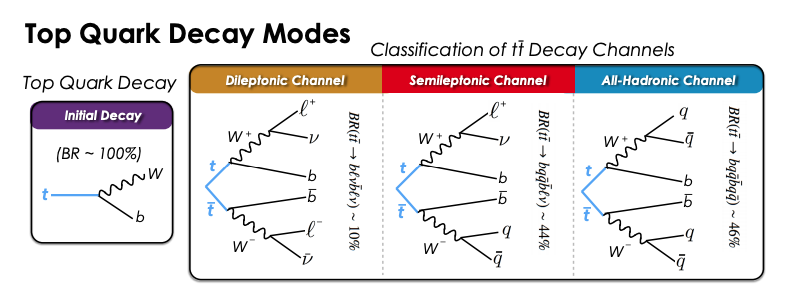
\includegraphics[width=0.8\linewidth]{Figures/ttbar-decay-mode.png}
	\caption{The schematic of Top quark decay channels.\cite{Mccarthy:2015ucy}}
	\label{fig:ttbardecaymode}
\end{figure}
\section{Machine Learning and its application on Particle Physics}

Machine Learning has been applied to most of the region in recent age, so dose particle physics. From the search of higgs boson(neural network and BDT) to the b-tagging technology(BDT\cite{Paganini:2017dpd}), physicist already applied several kinds of machine learning method to recent researchs.
\\
In a nutshell, machine learning can break into several cases, it can help to do classification, regression, and clustering problems. It can not only help to accelerate the computation of well-defined problems, and also find a new path to unsolved area. We will use a state-of-the-art machine learning technology, attention mechanism. The attention mechanism is a technology base on the evolution of RNN.\cite{A.Vaswani:2017} The attention mechanism will not only consider the local relationship and the sequence neighbor but also calculate the global relation base on the self-attention calculation shown in Figure \ref{fig:attention}. Using this novel architecture, we will train on the relationship between each jet and try to figure out the correct pair information.
\\
\begin{figure}[h]
	\centering
	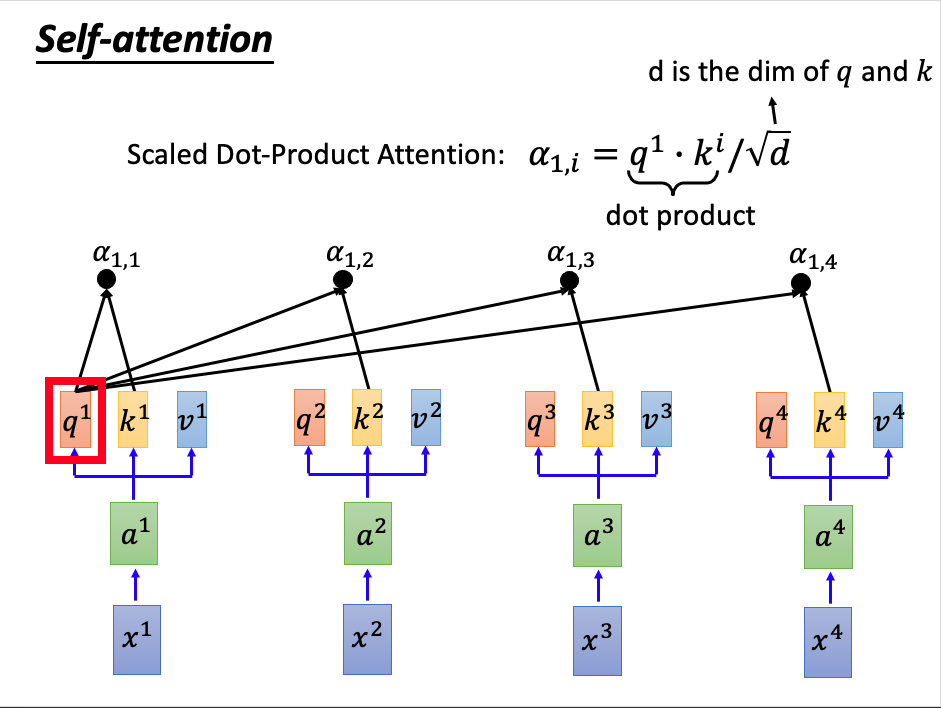
\includegraphics[width=0.8\linewidth]{Figures/attention.png}
	\caption{How self-attention works.\cite{HY.Lee:2019}}
	\label{fig:attention}
\end{figure}

\chapter{Event Generation}\label{Event Generation}

%This chapter is organized as follow. Section \ref{VBF:CommonSelection} provides ...


\section{MC samples}\label{sec:MC sample}
For data preparation, we generate our dataset using a custom docker image with MadGraph\_aMC@NLO(v2.7.2), Pythia8(v.8.2), and Delphes(v3.4.2) for showering, hadronization, and detector simulation. We apply the ATLAS parametrization during detector simulation.  The data are generated at Leading Order(LO) quantum chromodynamics(QCD) and using the PDF set NNPDF23\_lo\_as\_0130\_qed. The top mass is configured as $m_{\rm top}=173$ GeV. The W quark decay is forced hadronically into a $(q, q')$ pair. The following is our configuration:
\\
\begin{adjustbox}{max width=\textwidth}
\centering
\begin{lstlisting}[caption={Configuration for generating samples. The ``iseed'' is just a placeholder, it will be changed when generating samples.},captionpos=b]
	generate p p > t t~ QED=0, (t > W+ b, W+ > j j), (t~ > w- b~, w- > j j ) 
	output <file_path> 
	launch <file_path> 
	shower=Pythia8  
	detector=Delphes 
	analysis=OFF 
	done  
	set nevents = 10000 
	set iseed = 1 
	Delphes/cards/delphes_card_ATLAS.tcl
	done 
	exit 
\end{lstlisting}
\end{adjustbox}
\\
To get a more general performance, we scan the iseed value from 1 to 30000, each value has 10 thousand events before event selection. The reason for scanning iseed value is that the iseed value is the key to the random data generation. Originally, the program will choose the iseed value randomly and generate different samples. By scanning the issed value, we can make sure the seed is not reused. 






\chapter{Data analysis and Event reconstruction}\label{section:Reconstruction}


\section{Data analysis}\label{sec:Data analysis}
\subsection{Event selection}\label{subsec:Event selection}
The top all hadronic decay channel has 2 b-jets and 4 quark jets, all of them in our configuration is not in boosted region. Follow the event selection used in the reference\cite{Mccarthy:2015ucy},  we apply a event selection that an event should at least exists \textbf{2 b-jets} and \textbf{4 quark jets} satisfied $p_{T}$ larger than \textbf{25 GeV} and $|\eta|$ less than \textbf{2.5}. A cutflow table and figure can help us to understand how much events are killed by the selections. We may apply 5 cuts and see the evolution of survived event numbers. The rule of cuts is shown in Table \ref{table:cuts}, and the cutglow is shown in Figure \ref{fig:cutflow}. As the result, we found around 18\~20\% events will survived after the event selection. 

\begin{center}
	\begin{table}[h]
		\begin{tabular}{p{0.1\textwidth} c c c }
			\cline{1-3}
			\#Cut    & Number of b-jets & Number of quark jets  \\
			\hline
			C1      &   0  & 4    \\
			C2      &   0  & 5    \\
			C3      &   0  & 6    \\
			C4      &   1  & 6    \\
			C5      &   2  & 6    \\
			\hline
		\end{tabular}
		\caption{Rule of cuts. All the cuts require a kinematic limitation that $p_{T} > 25$ GeV and $|\eta|<2.5$.}
		\label{table:cuts}
	\end{table}
\end{center}

\begin{figure}[!h]
	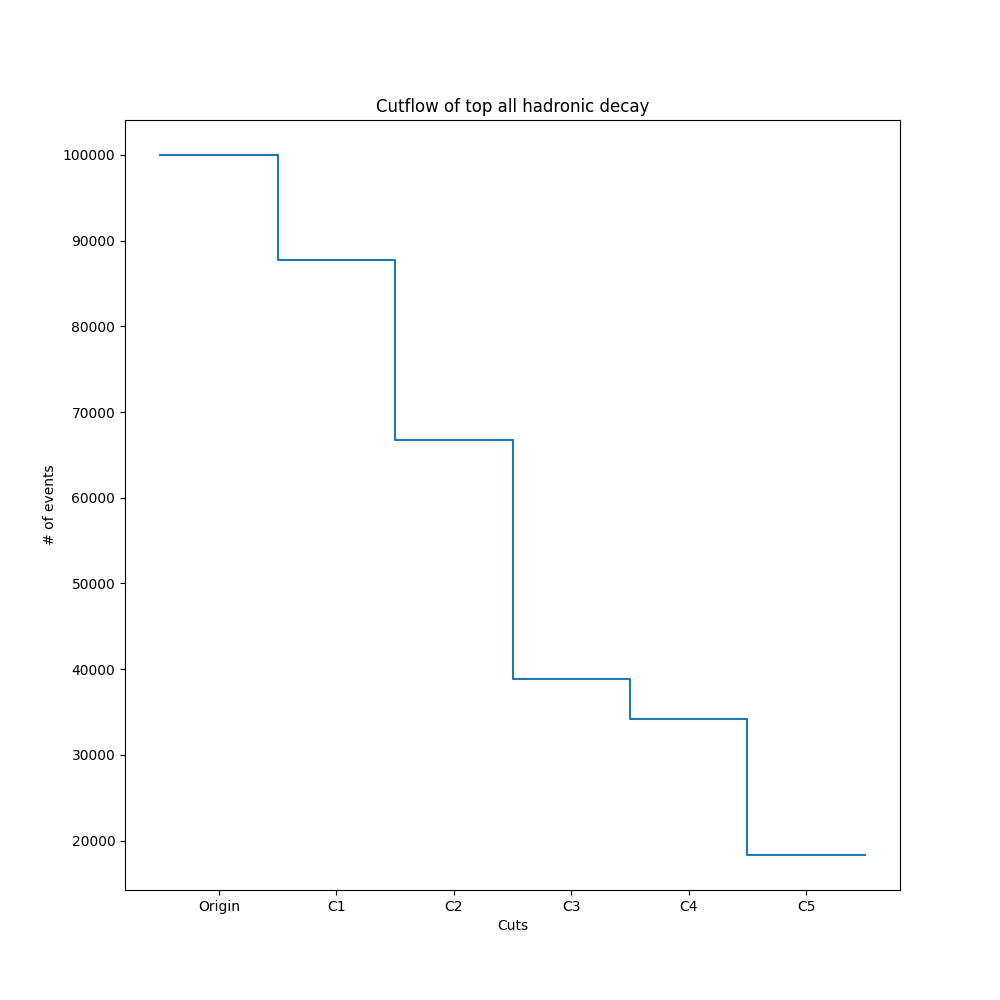
\includegraphics[width=0.8\linewidth, height=7cm,keepaspectratio=true]{Figures/ttbar_cutflow.png}
	\caption{Cutflow of all hadronic top decay.}
	\label{fig:cutflow}
\end{figure}
\begin{figure}[H]
	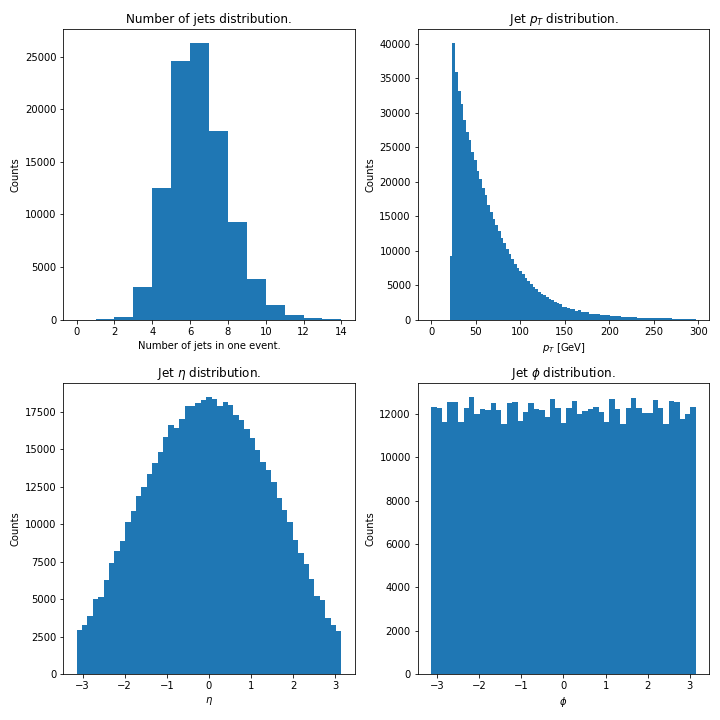
\includegraphics[width=0.8\linewidth, height=8cm,keepaspectratio=true]{Figures/ttbar_kinematic_dist.png}
	\caption{Demonstration of distributions.}
	\label{fig:kinematic dist}
\end{figure}
\newpage

\subsection{Truth matching}\label{subsec:Truth matching}
The \textbf{truth matching}, which is also called \textbf{$\Delta$R matching},  is to match the detector simulation(i.e. jet information generate by Delphes) data to truth record(i.e. parton level information).  To calculate the $\Delta R$ value, we will find the daughters of top quarks, W boson and b quark. After the daughters of top quarks is found, we will find the daughters of W bosons. After all, we will get six partons which are comes from the decay of top quark pairs. This six partons can match to the jets identically by considering their distances. The formula of calculating $\Delta R$ is:
\begin{equation}
	\Delta R = \sqrt{\Delta\eta^{2} + \Delta\phi^{2}}
\end{equation}
By using the kinematic properties provide in parton level and detector simulation information, we can calculate the the $\Delta R$ value between each parton and jets. After the calculation, we may assign each parton to a specific jet. 

\subsection{Custom barcode system}\label{subsec:barcode}
To specify the relation between each parton, and the relation between mothers and daughters, we design a barcode system which helps us to declare the relationship.

\begin{figure}[h!]
	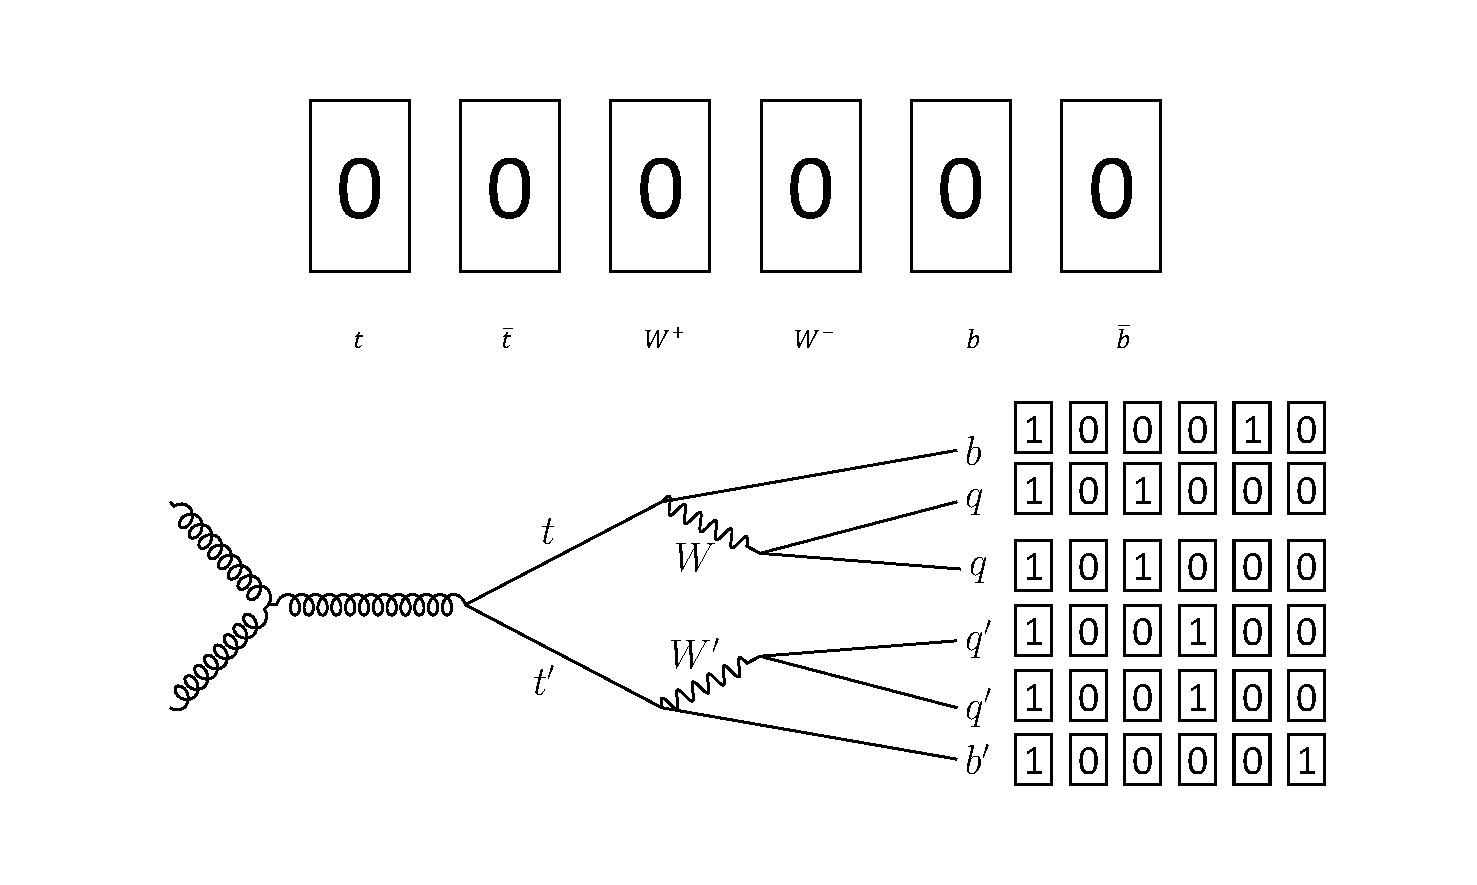
\includegraphics[width=0.8\linewidth]{Figures/barcode.pdf}
	\caption{Design of barcode.}
	\label{fig:barcode}
\end{figure}

As the 

\section{Event reconstruction}\label{sec:Event reconstruction}

\subsection{$\chi^{2}$ reconstruction}\label{subsec:chi-square}

\subsection{Machine Learning Approach}\label{subsec:ML approach}


%Section \ref{subsec:data_trigger} discusses the triggers used, the trigger efficiencies and the gains of signals with the current setup.
%\section{Common event selection}\label{VBF:CommonSelection}
...

%\begin{itemize}
%	\item Exactly two opposite charged and different flavor leptons ($e\mu+\mu e$)
%	\item $\pTlead > 22$ \gev, $\pTsublead > 15$ \gev
%	\item $\mll > 10$ \gev
%\end{itemize}



%\begin{table}[!h]
%	\centering
%	\caption{Ranking of the BDT training variables \cite{ATLASComNote}.}
%	\label{tab:ranking}
%	\scalebox{0.8}{
	%	\input{Figures/VBFAnalysis/BDTInput/ranking.tex}
%	}
%\end{table}



%\begin{table}[!h]
%	\centering
%	\caption{ 
	%	Event yields in the VBF SR after fitting. Event yields in the highest BDT bin are also presented. The uncertainties include systematic and statistical uncertainties \cite{HWWRun2Paper}.}
%	\label{tab:ggF_VBF_yields}
%	\scalebox{0.8}{
	%	\input{Figures/Cutflow/VBFanalysis/EventYieldVBF.tex}
%	}
%\end{table}





\chapter{Result and Discussion} \label{Discussion}

In this chapter, we will discuss our result and compare the performance between the traditional method and machine learning approach.

\section{Invariant mass and reconstruct efficiency }\label{sec:inv mass and reco eff}

Before discussing the result, we should define the category for the reconstruction efficiency. Treating the truth matching result as the target, the prediction of $\chi^{2}$ or SPA-NET may produce three kinds of results:

\begin{itemize}
	\item Correct matched: An event that both top quarks are correctly predicted by the reconstruction method.
	\item Incorrect matched: An event that one or both top quarks is incorrectly predicted by the reconstruction method.
	\item Unmatched: An event that one of the truth match results contains an element that does not match to any jets.
\end{itemize}
Based on the category above, we can compute the reconstruction efficiency. For the reconstruction efficiency, we separate it into two parts: event-based efficiency and quark-based efficiency. For event-based efficiency, we will calculate the efficiency base on how many \textbf{events} are matched correctly, incorrectly, and unmatched. Meanwhile, the quark-based efficiency calculates the efficiency base on how much \textbf{top quarks} are assigned correctly. The efficiency is shown in the table below:
\\
\begin{table}[H]
	%\captionsetup{justification=raggedright,singlelinecheck=false}
	\caption{Using $\epsilon$ as the symbol of efficiency. This table performs the efficiencies of the $\chi^2$ and SPA-NET assignments assessed by per-event efficiency $\epsilon^{event}$ and per-top efficiencies $\epsilon^{top}$ inclusively and by jet multiplicity \Njets. The subscript of $\epsilon^{top}_{1}$ and $\epsilon^{top}_{2}$ is stands for the one/two reconstructable events.}
	\centering
	\begin{tabular}{c c  c  c  c c  c}
		\hline
		\hline
		& \multicolumn{3}{c}{$\chi^2$ Method} & \multicolumn{3}{c}{SPA-NET }\\
		\hspace{0.2cm}\Njets & \hspace{0.15cm} \epsevent & $\epstoptwo$ & \hspace{0.15cm} $\epstopone$ \hspace{0.15cm} & \hspace{0.15cm} \epsevent & $\epstoptwo$ & \hspace{0.15cm} $\epstopone$ \hspace{0.15cm}   \\
		\midrule
		6          & 61.8\% & 65.0\% & 24.2\% & 80.7\% & 84.1\% & 56.7\% \\
		7          & 40.8\% & 50.4\% & 24.6\% & 66.8\% & 75.7\% & 56.2\% \\
		$\geq$8    & 23.2\% & 35.5\% & 20.2\% & 52.3\% & 66.2\% & 52.9\% \\
		\midrule     
		\vspace{0.2cm}
		\textbf{Inclusive}  &\textbf{ 37.7}\% & \textbf{47.0}\% & \textbf{23.0\%} & \textbf{63.7}\% &\textbf{73.5}\% &\textbf{55.2\%} \\
		\hline
	\end{tabular}
	\label{tab:eps}
\end{table}
The $\chi^{2}$ has performed a $37.7\%$ efficiency on overall events, while SPA-NET archives an efficiency $63.7\%$. The $\chi^{2}$ method has the best performance on the 6 jets category and has the worst effort on the category that an event contains more than 8 jets. The SPA-NET perform much better the $\chi^{2}$ in all category. For the event that contains two identifiable, the $\chi^{2}$ method achieves an efficiency $\epsilon^{top}_{2}$ $65.0\%$, and SPA-NET archives an $\epsilon^{top}_{2}$ $84.1\%$. Since we train the SPA-NET we the events that contain two top quarks, it is reasonable that the $\epsilon^{top}_{1}$ of SPA-NET is lower than $\epsilon^{top}_{2}$. Also, since our definition of equation \ref{eqn:chi2} is base on the difference between reconstructing invariant mass of 2 two quark candidates, so an event that only contains one identifiable top quark, is hard for $\chi^{2}$ method to assign the jet properly. Note that in our evaluation dataset, 8.1\% of events in which both tops are identifiable have at least one $b$-quark matched to non-$b$-tagged jets. These quarks, which are impossible for our $\chi^2$ to correctly reconstruct, are reconstructed by SPA-NET with an efficiency of 29.4\%. 

\subsection{Reconstructed invariant mass }\label{subsec:reco inv mass }

Using $\chi^{2}$ minimization, we may obtain the best assignment under the constraint of parameters. In this project, the parameters are configured as: $m_{W}=81.3$ GeV, $\sigma_{W} = 12.3$ GeV, and $\sigma_{m_{bjj}}=26.3$ GeV. The parameters $\sigma_{W}$ and $\sigma_{m_{bjj}}$ are found by fitting the mass distribution of W boson and top quark. While computing $\chi^{2}$ value, we use the b-tagging information to assign the b quark candidates. 
\\
Following is the reconstructed mass distribution of W boson and top quark using $\chi^{2}$ minimization method and SPA-NET.
\\
\begin{figure}[H]
	\centering
	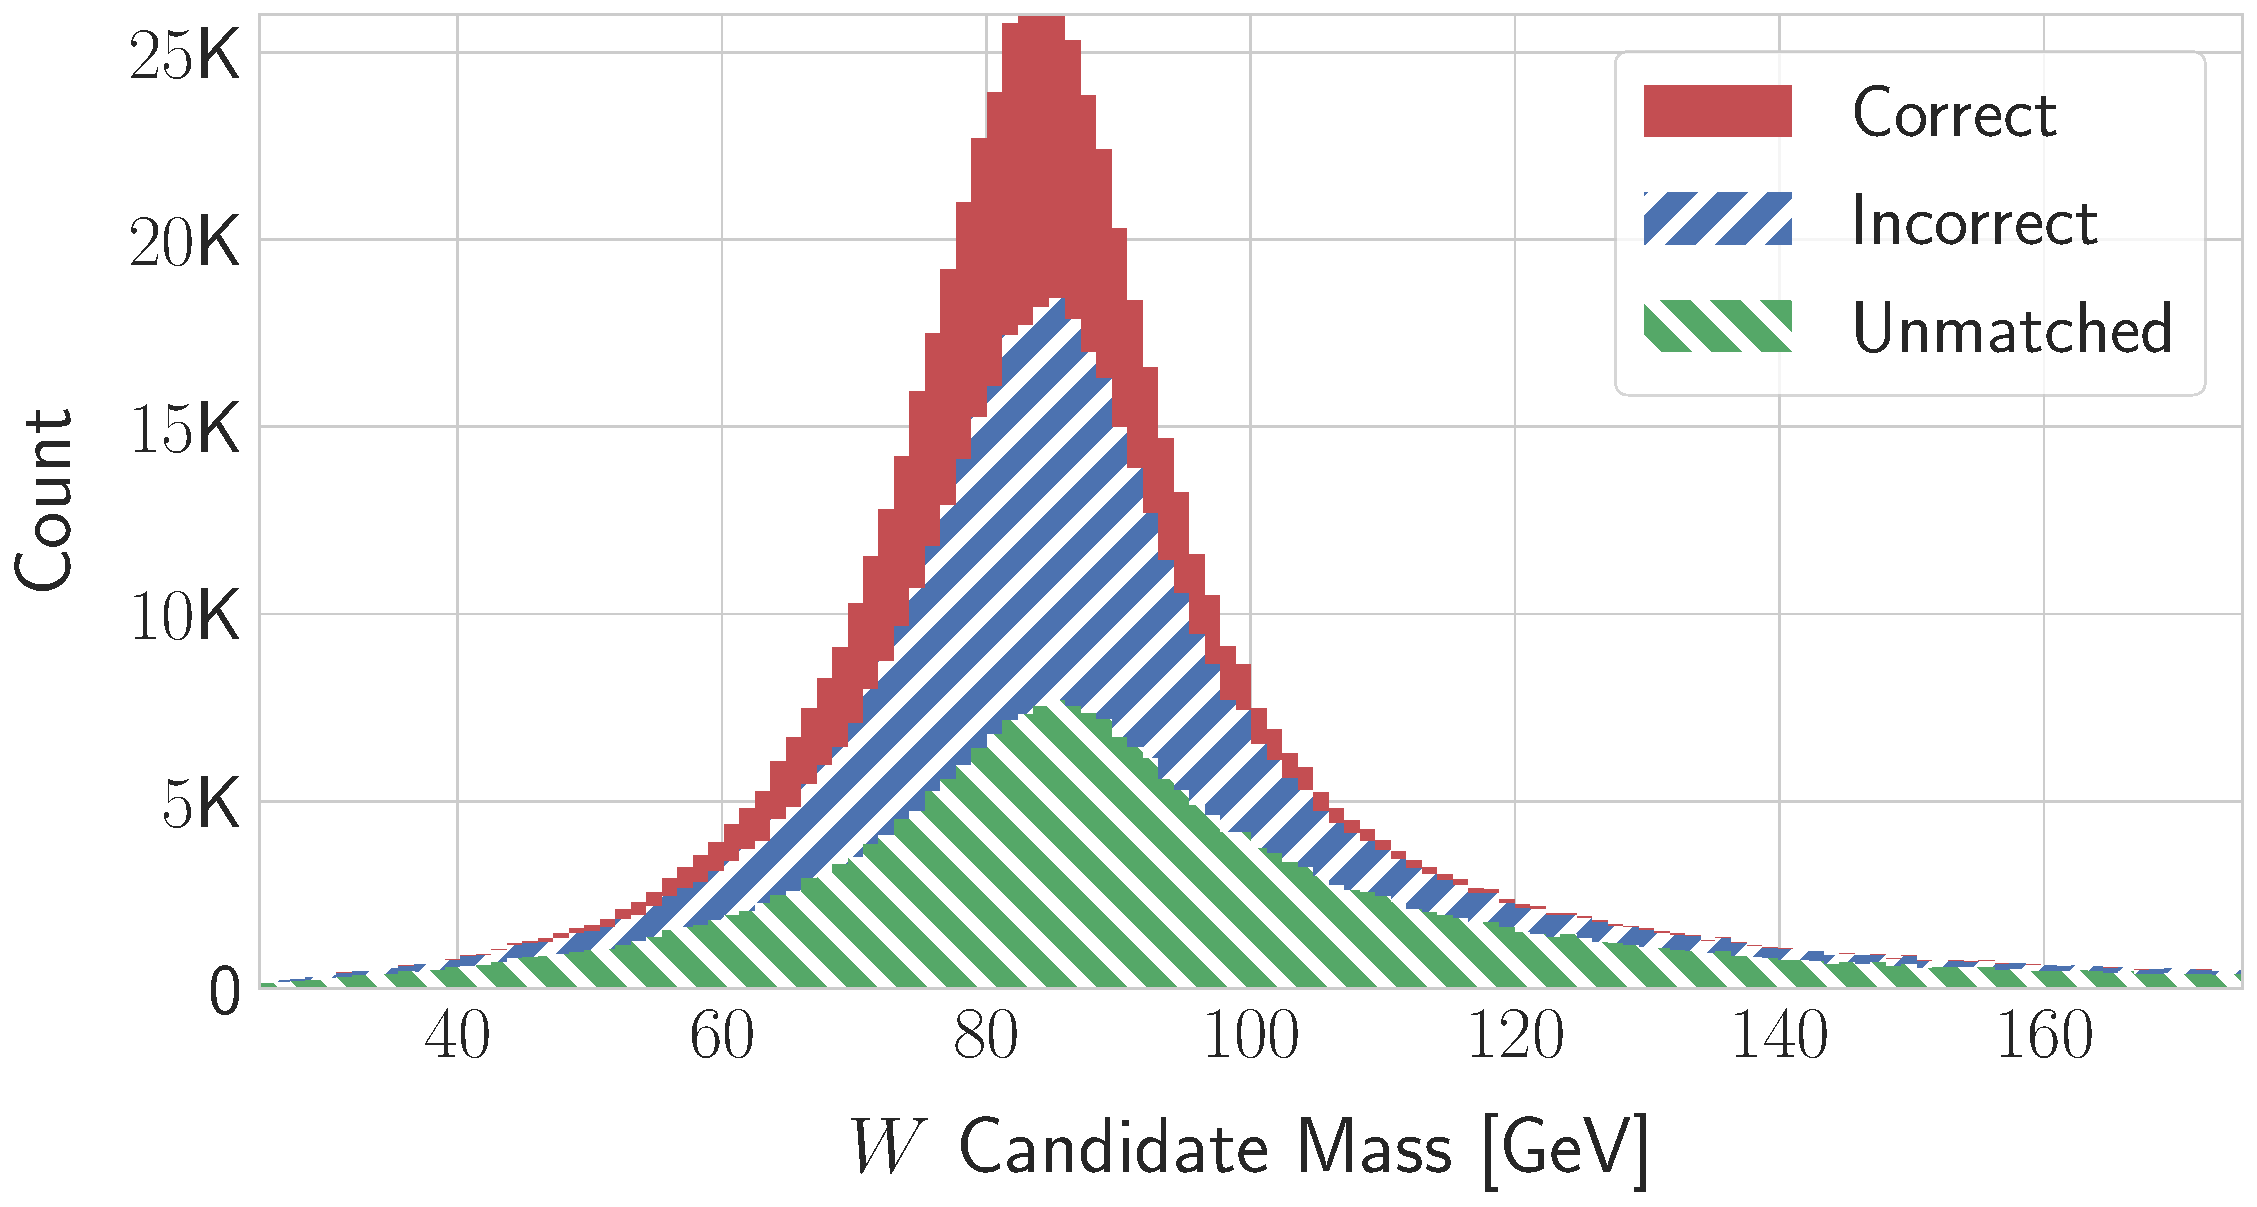
\includegraphics[width=0.7\textwidth]{Figures/network_w_quark_stacked_chi2.pdf}
	\caption{W boson mass reconstructed by $\chi^{2}$ minimization method}
	\label{fig: chi2 reco Wboson}
\end{figure}
\begin{figure}[H]
	\centering
	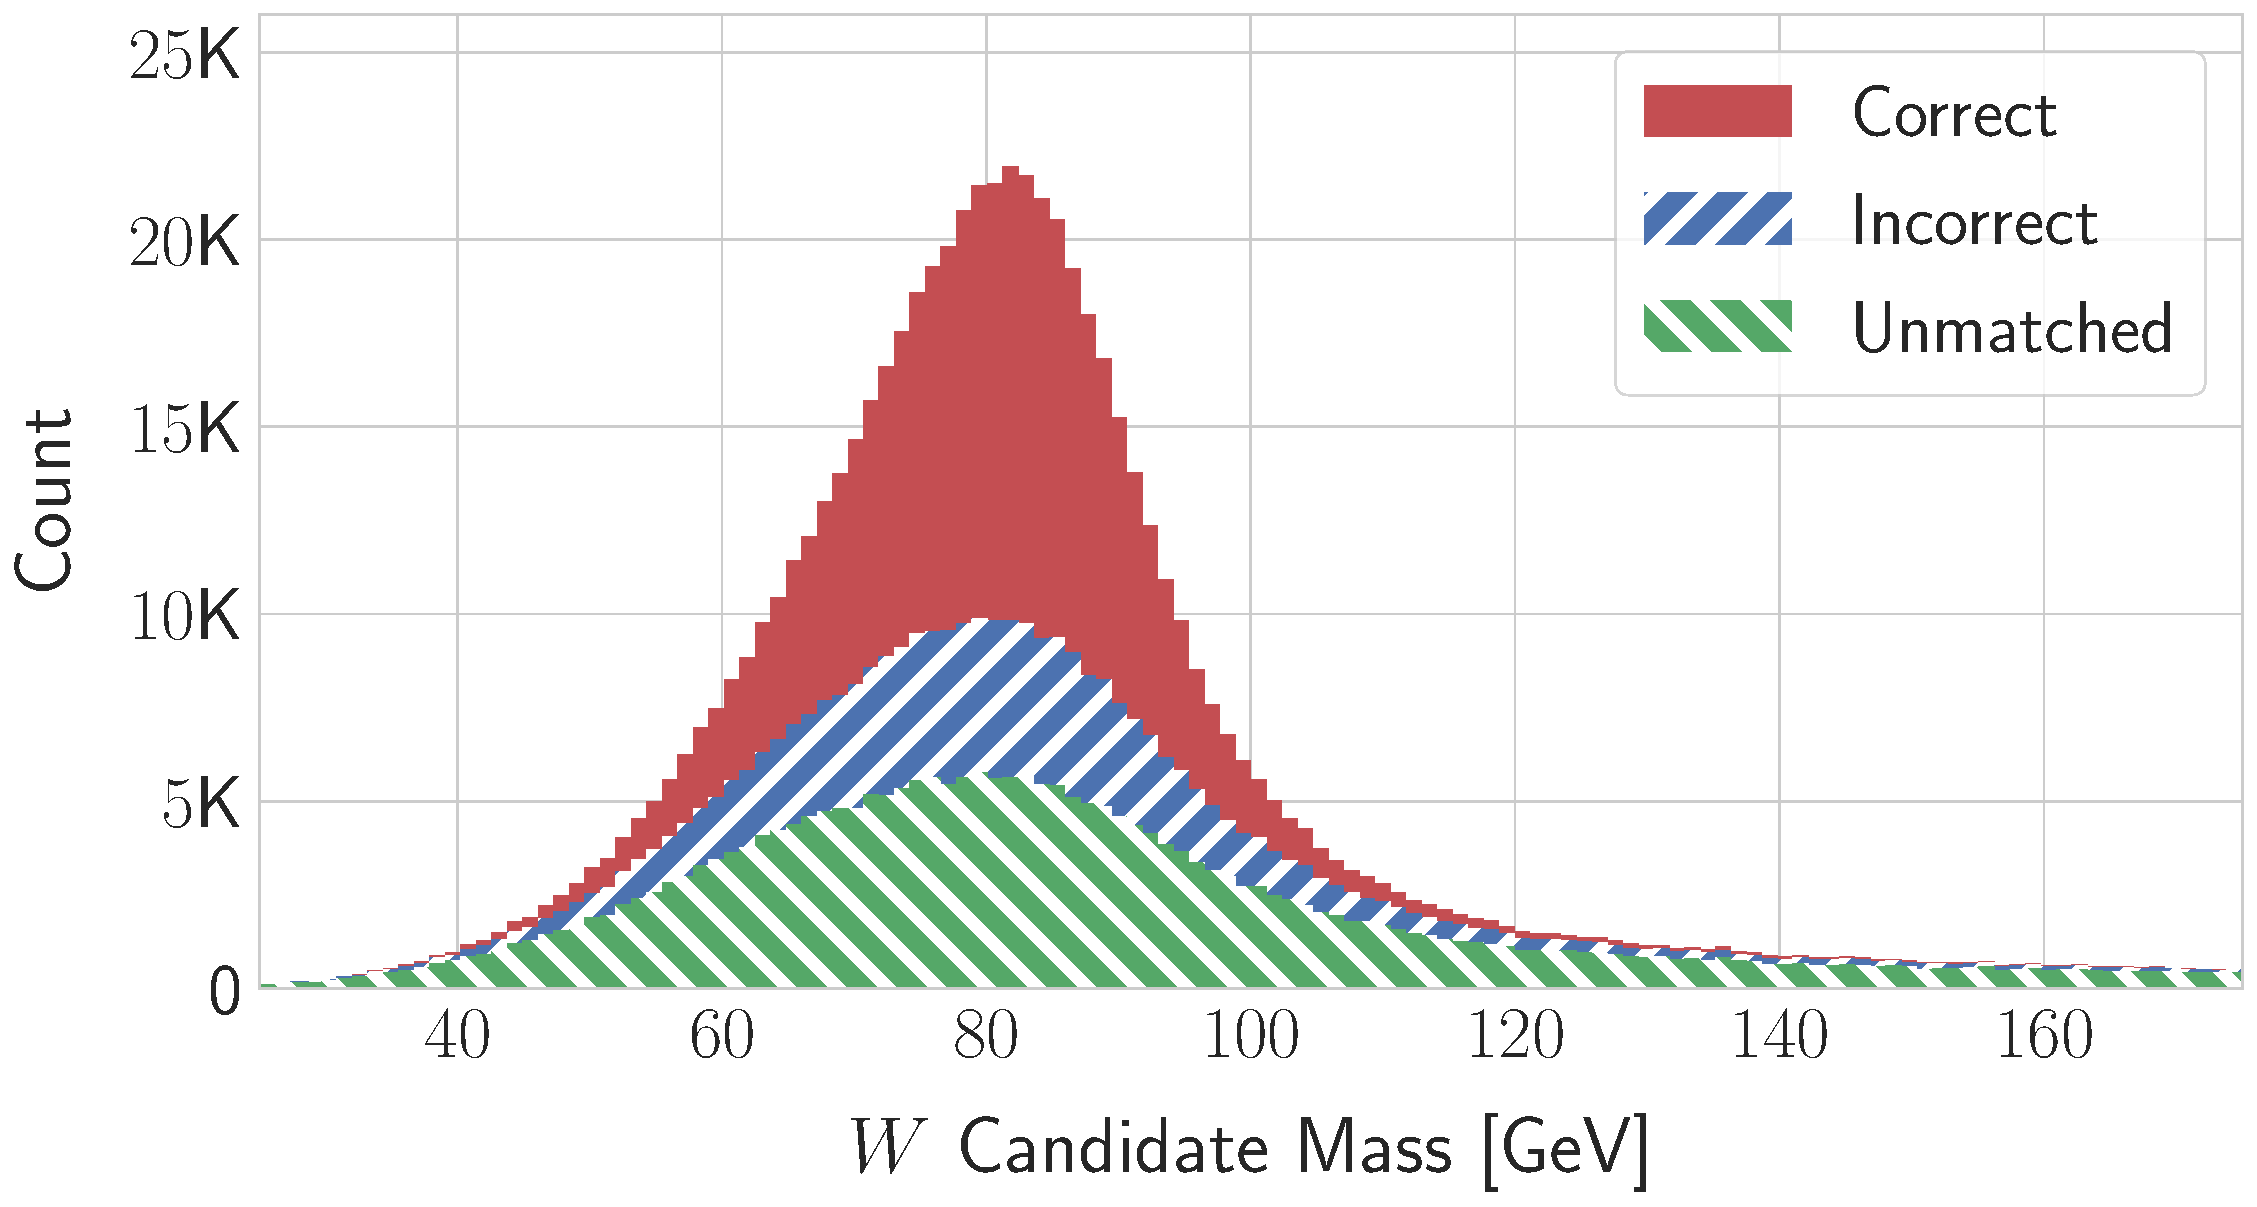
\includegraphics[width=0.7\textwidth]{Figures/network_w_quark_stacked.pdf}
	\caption{W boson mass reconstructed by SPA-NET}
	\label{fig: spanet reco Wboson}
\end{figure}

\begin{figure}[H]
	\centering
	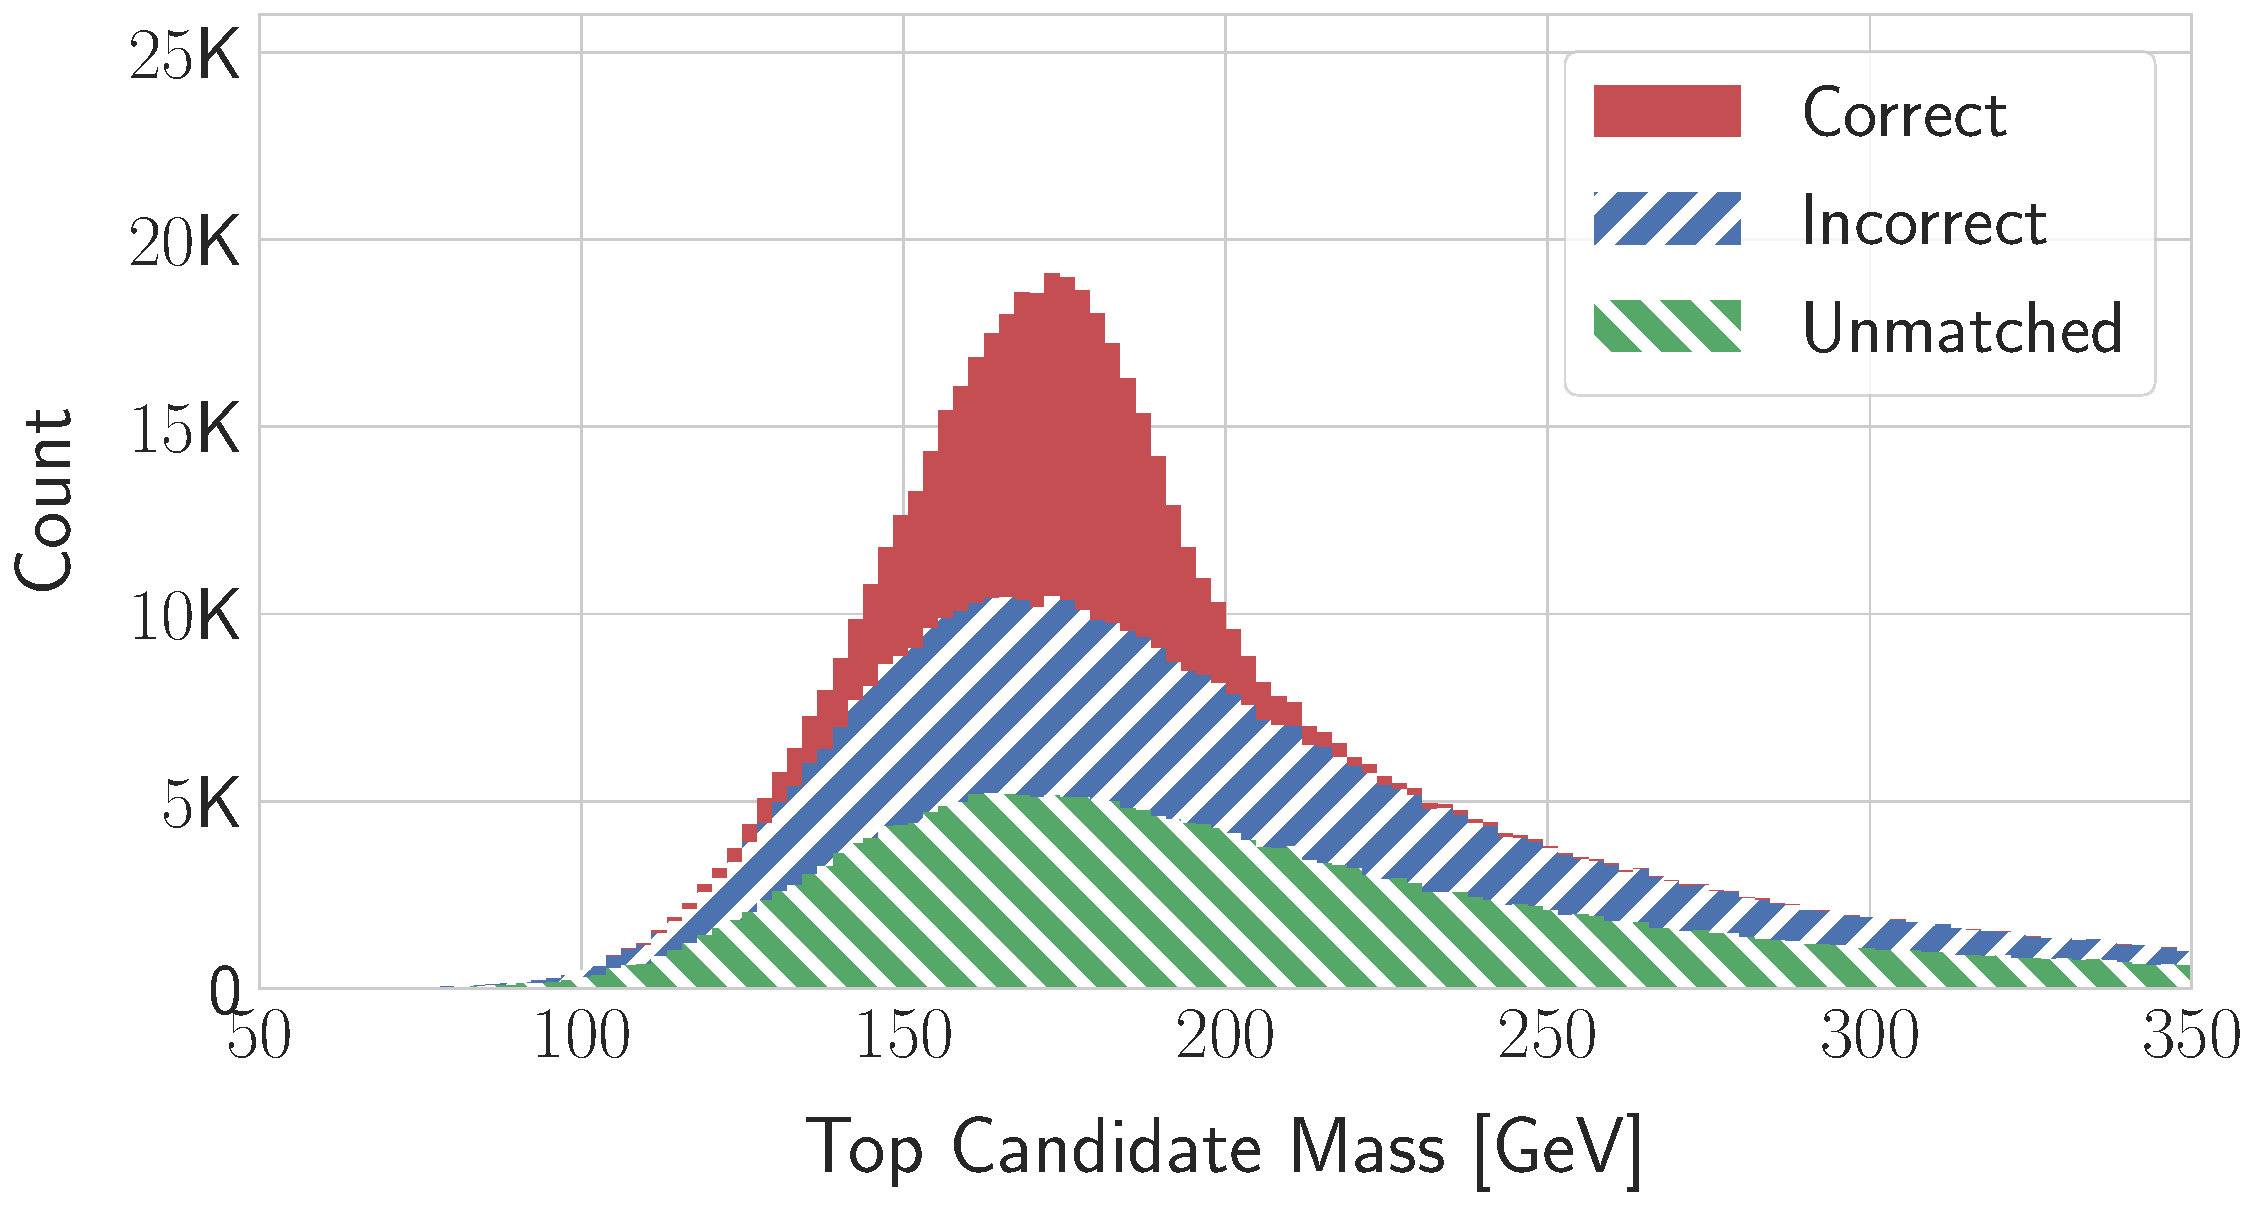
\includegraphics[width=0.7\textwidth]{Figures/network_t_quark_stacked_chi2.pdf}
	\caption{ Top quark mass reconstructed by $\chi^{2}$ minimization method}
	\label{fig: chi2 reco t quark}
\end{figure}
\begin{figure}[H]
	\centering
	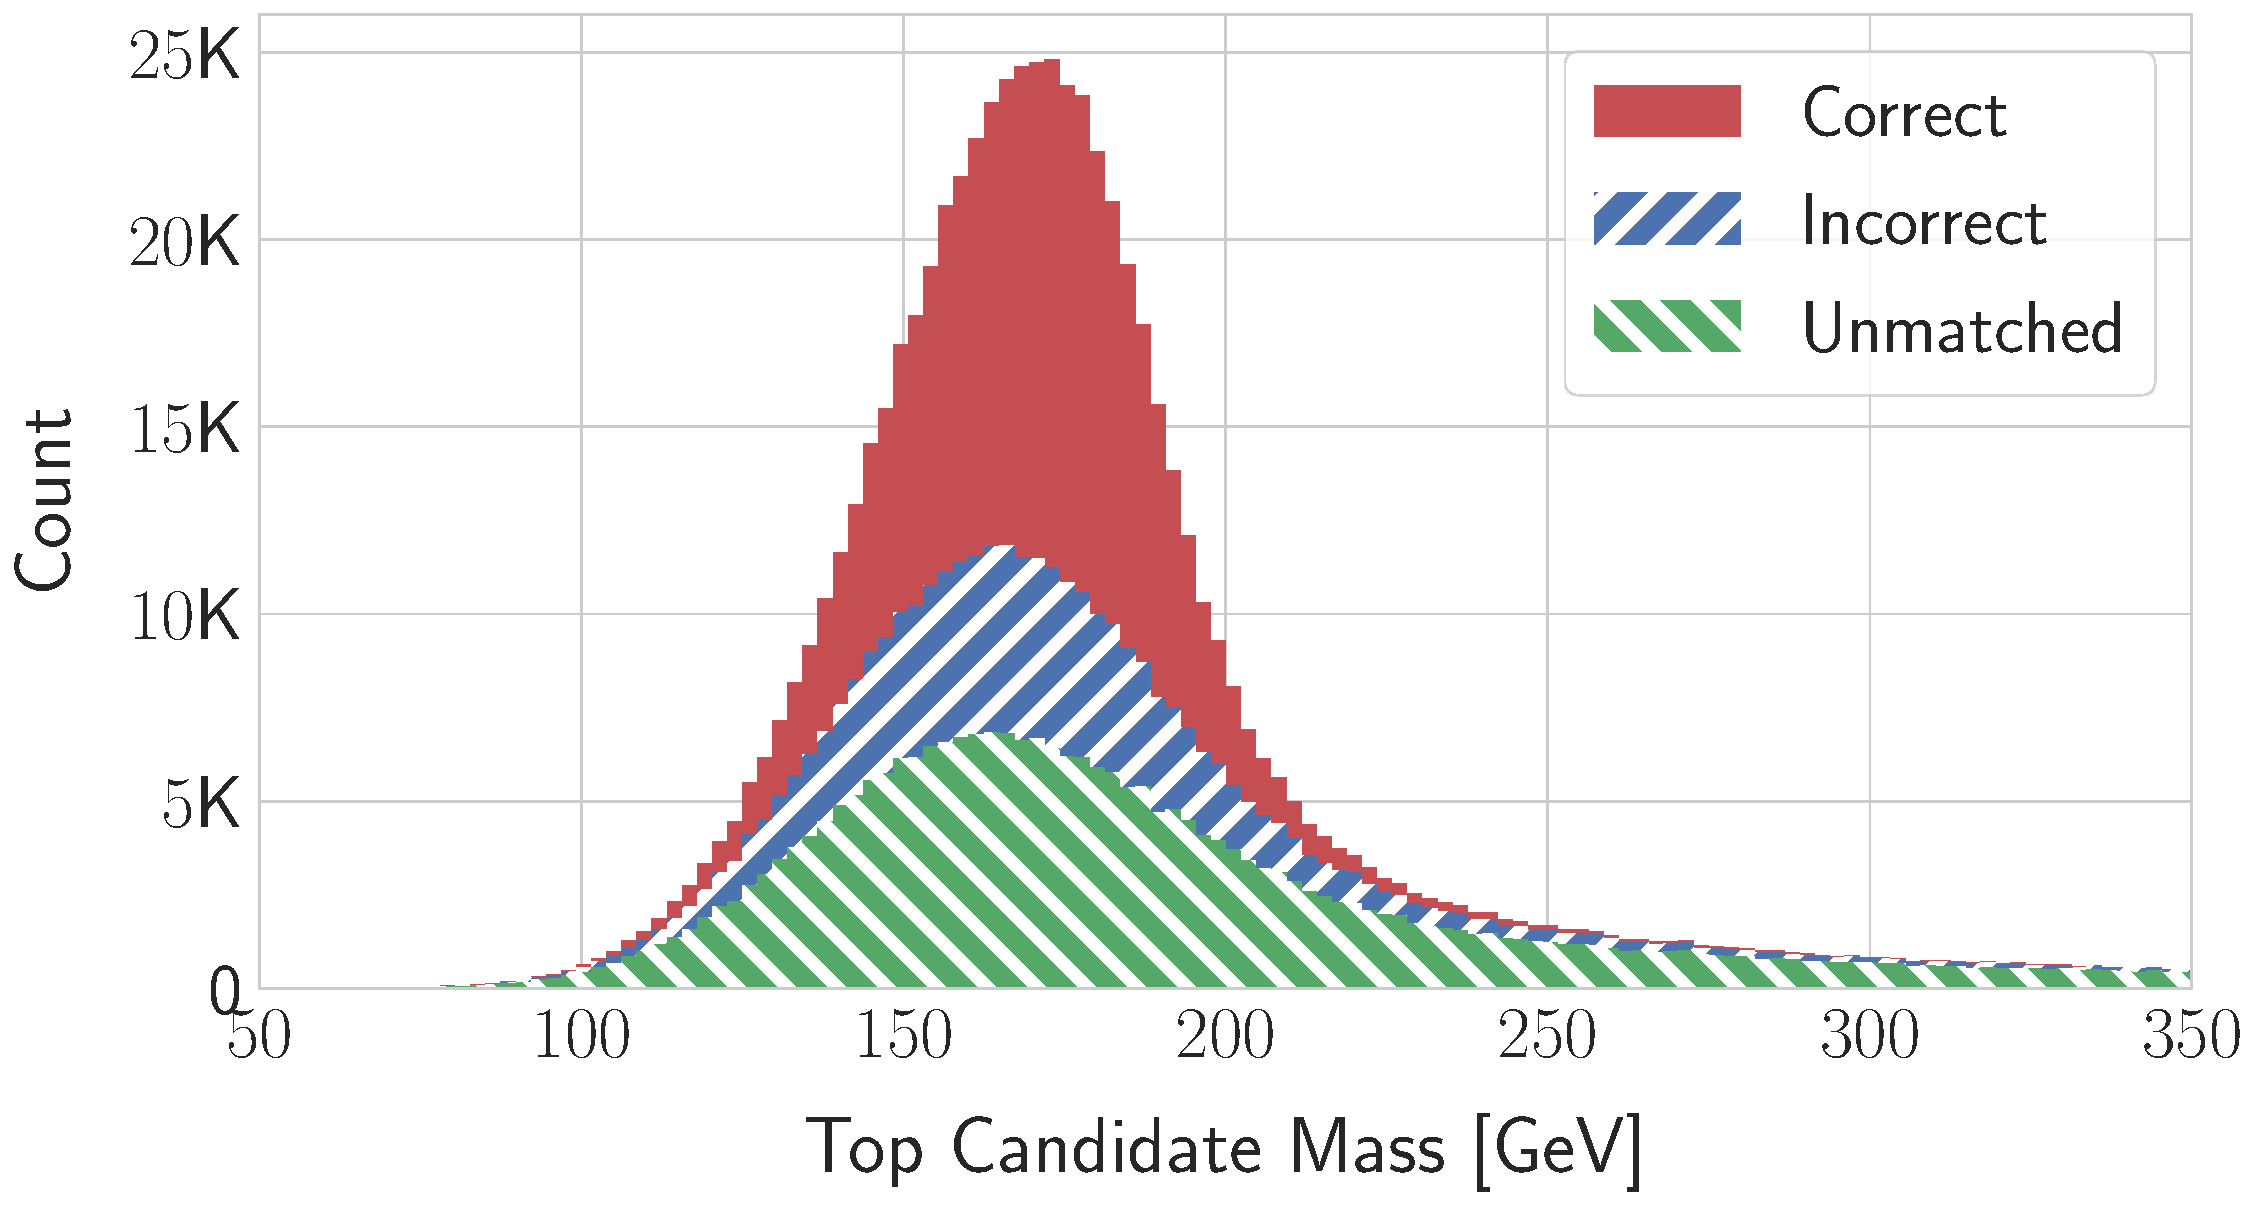
\includegraphics[width=0.7\textwidth]{Figures/network_t_quark_stacked.pdf}
	\caption{ Top quark mass reconstructed by SPA-NET}
	\label{fig: spanet reco t quark}
\end{figure}
Comparing the result shown in Figure \ref{fig: chi2 reco Wboson} and Figure \ref{fig: spanet reco Wboson}, we found the $\chi^{2}$ method has a narrower peak around W boson mass than the SPA-NET. This shape comes from the incorrect and unmatched events and can be explained by the presence of $m_{W}$ in equation \ref{eqn:chi2}. Another point is the Figure \ref{fig: spanet reco t quark} and Figure \ref{fig: chi2 reco t quark} shows that the SPA-NET has the more peaked distribution compare to $\chi^{2}$ method with comparable incorrect/unmatched events.

\subsection{ROC curve}\label{sebsec:roc}
The Receiver operating characteristic (ROC) curve is a good target to estimate the performance of a machine learning model. The ROC curve of SPA-NET apply on events with one and two reconstructable top quarks is shown in Figure \ref{fig: roc one top} and Figure \ref{fig: roc two top}. Note that the targets are defined as 1 if the prediction is correct, otherwise the 0 represents the incorrect prediction.
\\
 \begin{figure}[H]
 	\centering
 	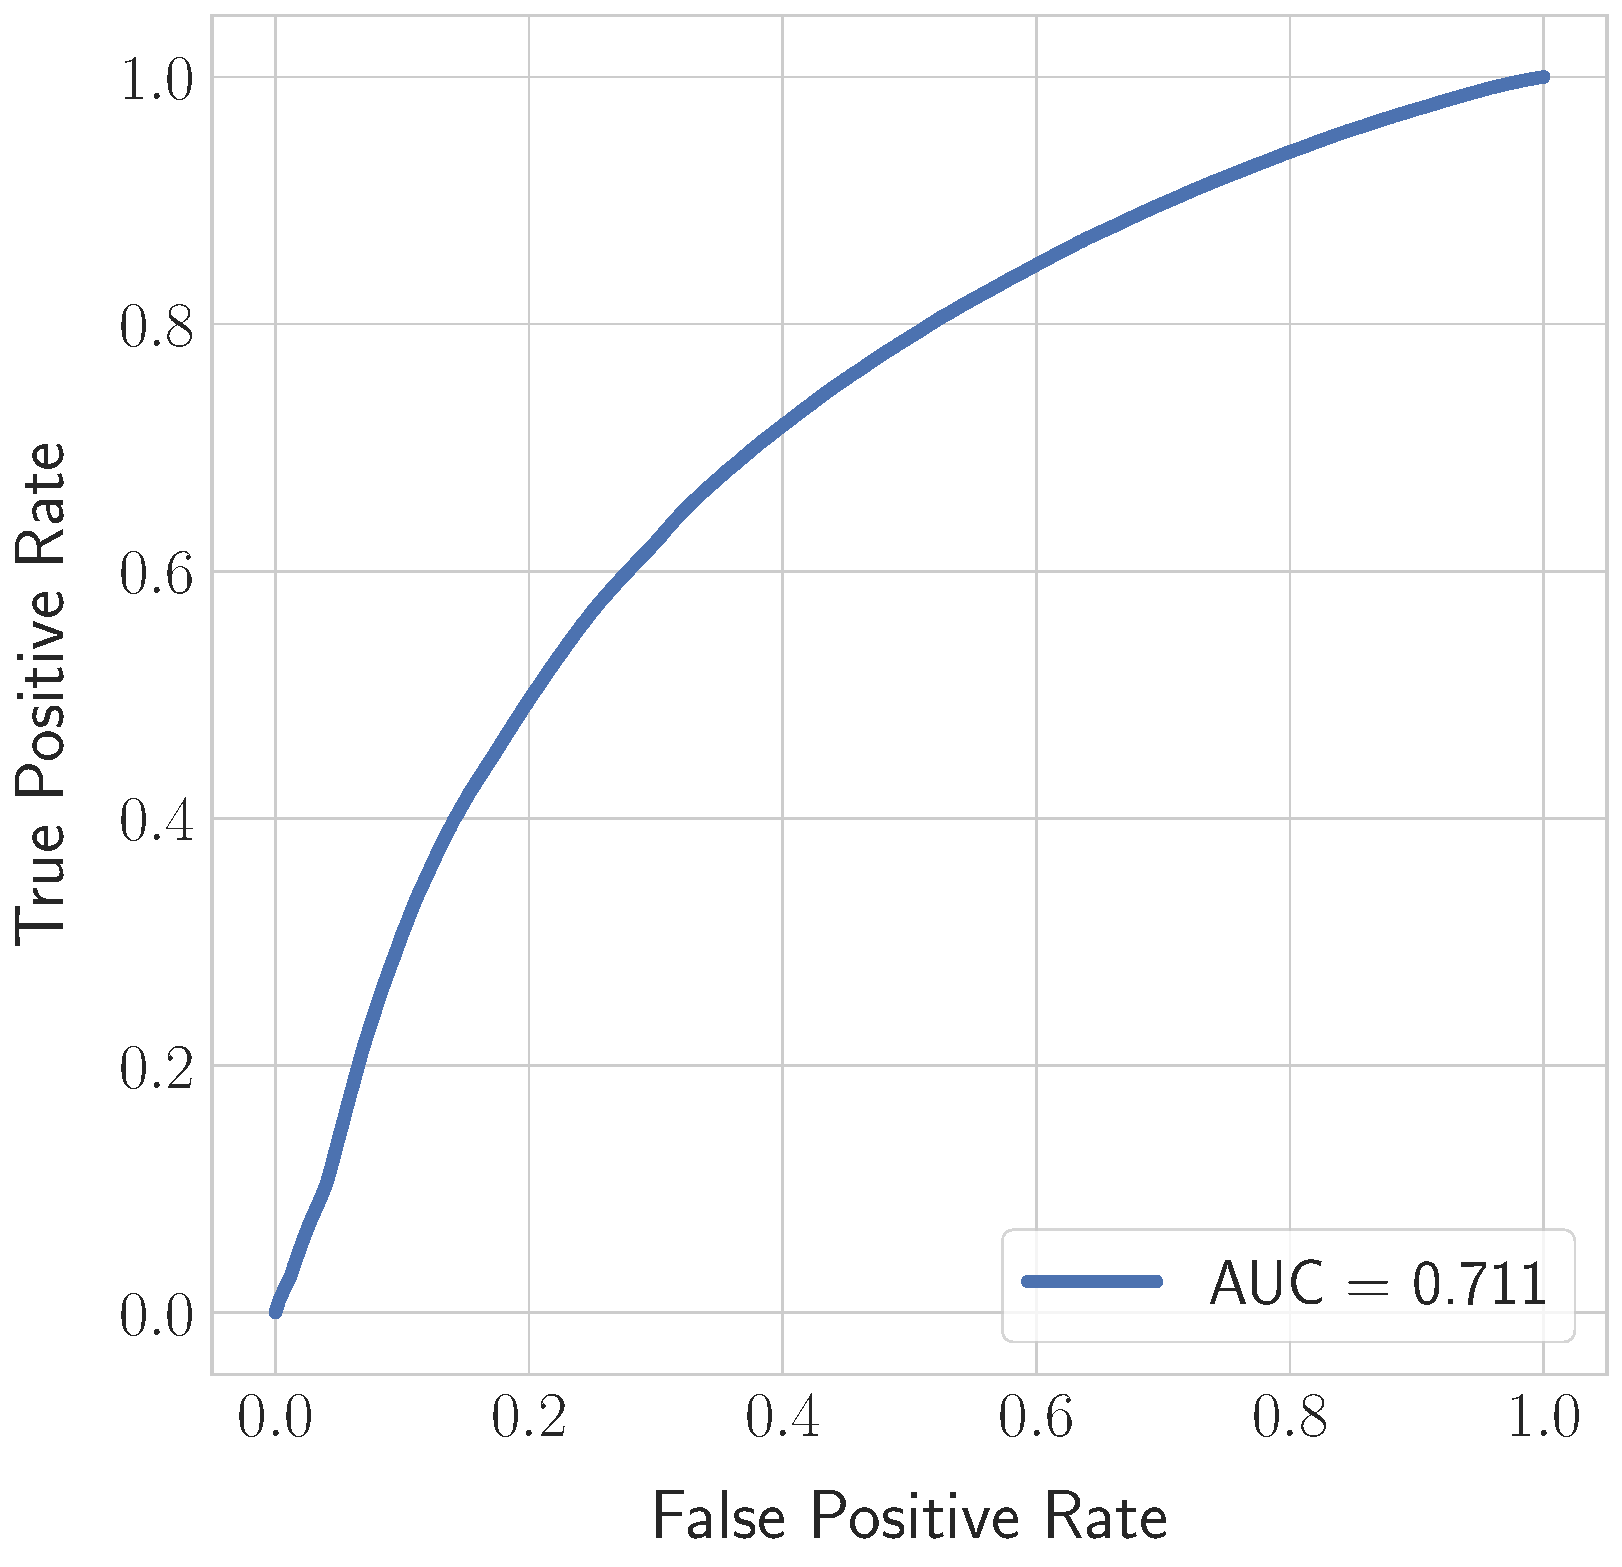
\includegraphics[width=0.6\textwidth]{Figures/roc_one_quark.pdf}
 	\caption{ ROC curve of SPA-NET apply on events with one reconstructable top.}
 	\label{fig: roc one top}
 \end{figure}
 \begin{figure}[H]
 	\centering
 	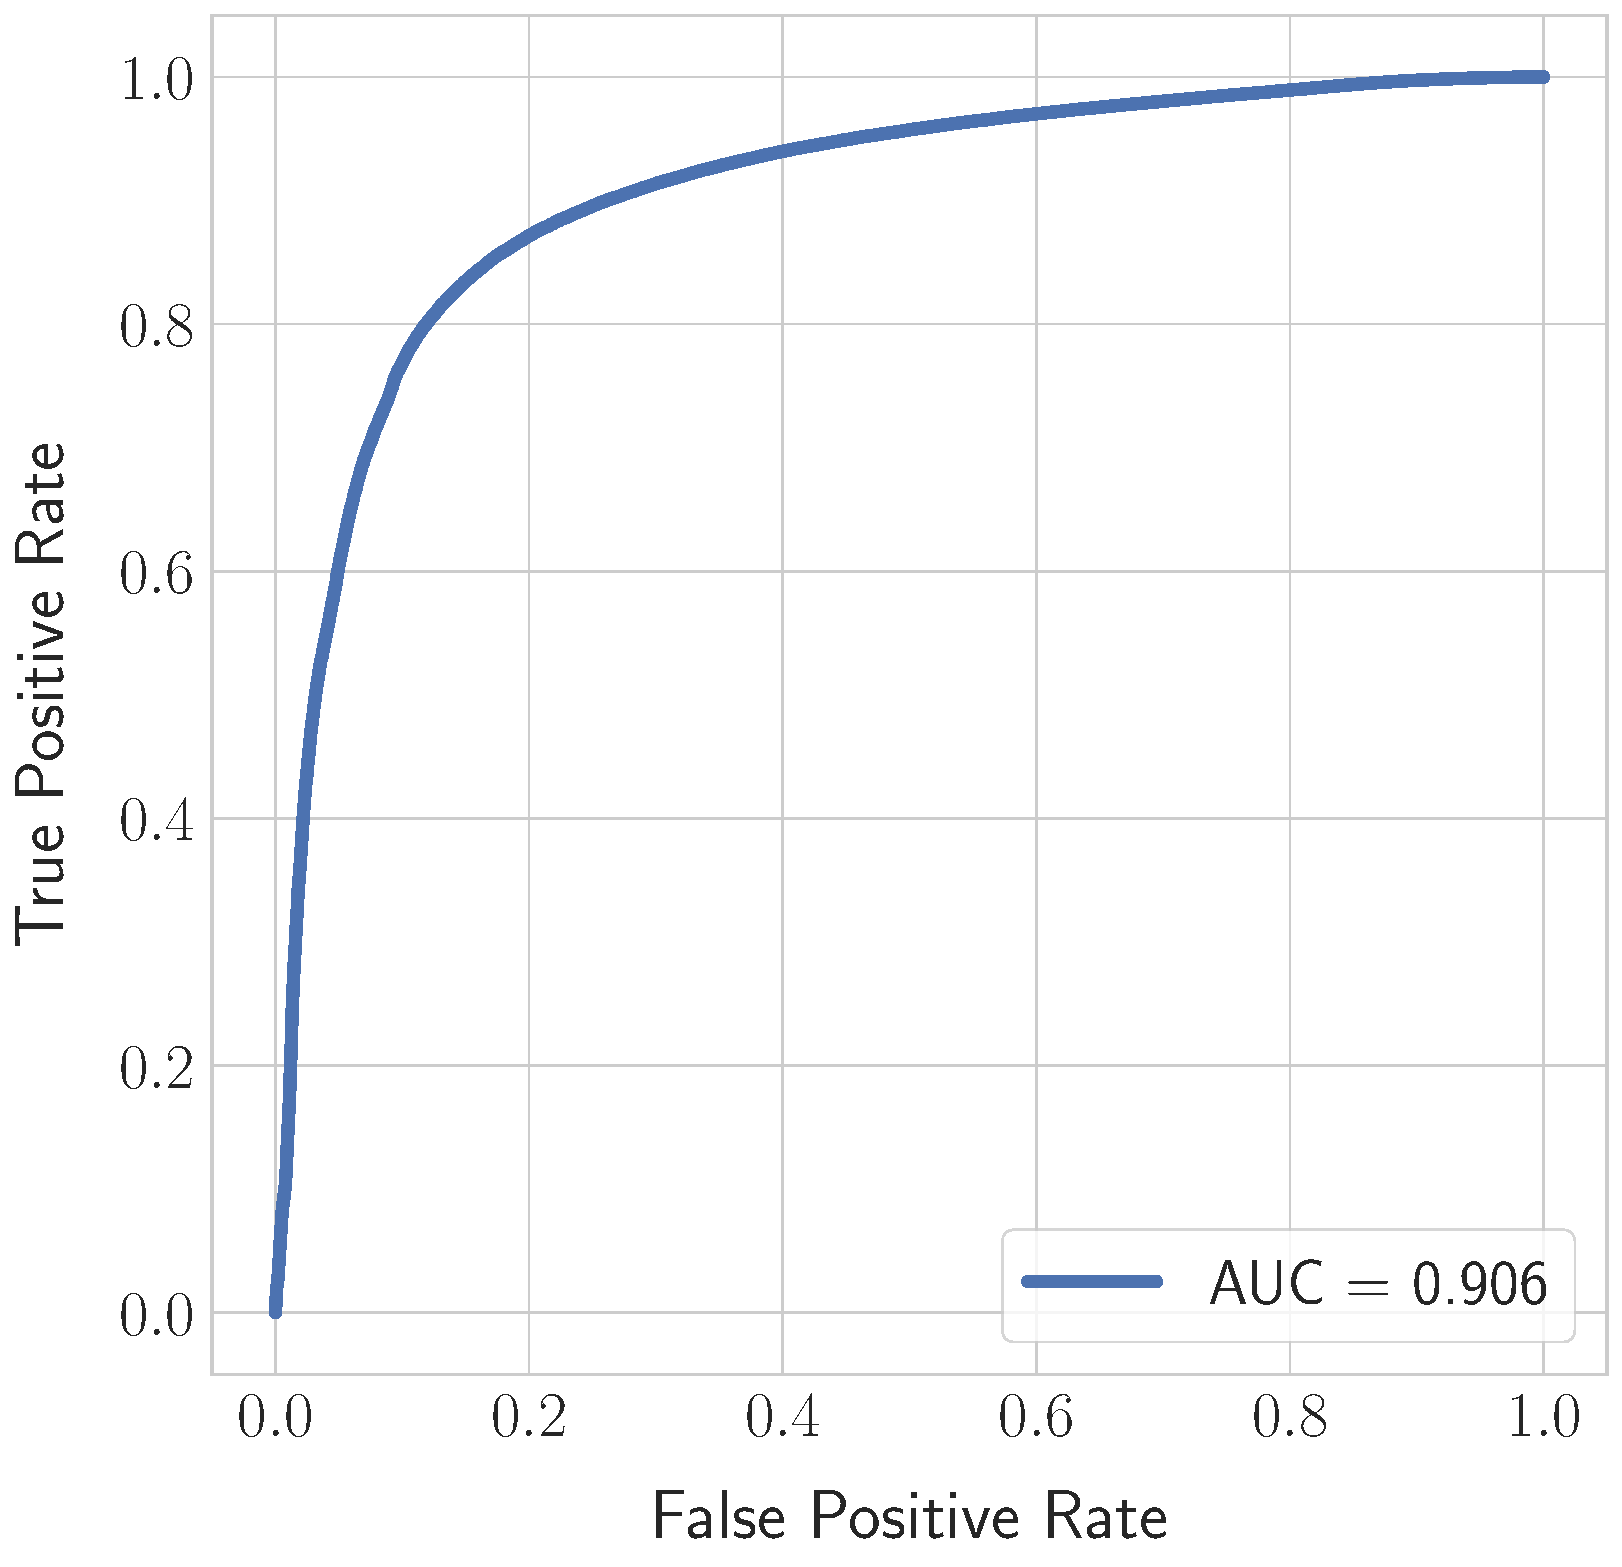
\includegraphics[width=0.6\textwidth]{Figures/roc_two_quark.pdf}
 	\caption{ ROC curve of SPA-NET apply on events with two reconstructable top.}
 	\label{fig: roc two top}
 \end{figure}
\newpage
As the advantage we discuss in the last paragraph of section \ref{sec:inv mass and reco eff}, our network archieves a lower AUC value in Figure \ref{fig: roc one top} and perform a remarkable ROC curve in Figure \ref{fig: roc two top}. A possible solution we haven't implemented in this report is to train with the ``partial'' events by using the ``mask''.\cite{Fenton:2020woz}\cite{Shmakov:2021qdz}
\section{Reduce of time usage}\label{sec: reduce of time uasge}
The time required to compute SPA-NET is much lower than the $\chi^{2}$ needed. We may compare the time they needed by considering the time complexity. The $\chi^{2}$ has a time complexity scales approximately as $P(N,6)=\mathcal{O}(N^{6})$ where N is the number of jets in an event. The time complexity is $\chi^{2}$ proportional to the number of jets and this makes a limitation of maximum jets is indeed. Consider a 2019 DELL XPS13 computer with Core i7-1065G7 1.30GHz CPU, the SPA-NET took an average of 4.4 ms for one event.  The $\chi^{2}$ took an average 20 ms in 6 jets events and 369 ms in $\ge$ 8 jets events. 
\section{Outlook}\label{sec:outlook}
Based on the design of SPA-NET, the input is a sequence of jets information and their relationships. The network consider the permutation relation between each subset and possible permutations. In case, a physics model which has a permutation relationship might be a good item to explore with SPA-NET. For example, $ttH$ all hadronic decay process or all hadronic four top decay process is a potential target to study with SPA-NET. Further more, not only the parton-jet assignment problem but also the clustering problem, graph matching problem, and so does other problem which contains a permutaion symmetry, is a potential item to study with SPA-NET. We plan to explore the SPA-NET with some interesting BSM problem, such as the tri-Higgs production in 2HDM model.\cite{Low:2020iua}




\chapter{Conclusion}

\begin{thebibliography}{99}
\addcontentsline{toc}{chapter}{Reference}  % Add "Reference" into the table of contents

%\cite{Aad:2012tfa}
\bibitem{Aad:2012tfa}
G.~Aad \textit{et al.} [ATLAS],
``Observation of a new particle in the search for the Standard Model Higgs boson with the ATLAS detector at the LHC,''
Phys. Lett. B \textbf{716}, 1-29 (2012)
doi:10.1016/j.physletb.2012.08.020
[arXiv:1207.7214 [hep-ex]].
%12265 citations counted in INSPIRE as of 24 May 2021

%\cite{Chatrchyan:2012ufa}
\bibitem{Chatrchyan:2012ufa}
S.~Chatrchyan \textit{et al.} [CMS],
``Observation of a New Boson at a Mass of 125 GeV with the CMS Experiment at the LHC,''
Phys. Lett. B \textbf{716}, 30-61 (2012)
doi:10.1016/j.physletb.2012.08.021
[arXiv:1207.7235 [hep-ex]].
%11972 citations counted in INSPIRE as of 24 May 2021

\bibitem{A.Vaswani:2017}
A.~Vaswani \textit{et al.},
``Attention is all you need,''
Advances in Neural Information Processing Systems, NIPS (2017)

%\cite{Zyla:2020zbs}
\bibitem{Zyla:2020zbs}
P.~A.~Zyla \textit{et al.} [Particle Data Group],
%``Review of Particle Physics,''
PTEP \textbf{2020}, no.8, 083C01 (2020)
doi:10.1093/ptep/ptaa104
%1494 citations counted in INSPIRE as of 04 Jun 2021

\bibitem{A.Quadt:2008TopPhysics}
A.~Quade,
``Top quark physics at hadron colliders,"
doi:10.1007/978-3-540-71060-8

%\cite{Sirunyan:2018mlv}
\bibitem{Sirunyan:2018mlv}
A.~M.~Sirunyan \textit{et al.} [CMS],
``Measurement of the top quark mass in the all-jets final state at $\sqrt{s} =$ 13 TeV and combination with the lepton+jets channel,''
Eur. Phys. J. C \textbf{79}, no.4, 313 (2019)
doi:10.1140/epjc/s10052-019-6788-2
[arXiv:1812.10534 [hep-ex]].
%40 citations counted in INSPIRE as of 04 Jun 2021

%\cite{Aaboud:2017mae}
\bibitem{Aaboud:2017mae}
M.~Aaboud \textit{et al.} [ATLAS],
``Top-quark mass measurement in the all-hadronic $ t\overline{t} $ decay channel at $ \sqrt{s}=8 $ TeV with the ATLAS detector,''
JHEP \textbf{09}, 118 (2017)
doi:10.1007/JHEP09(2017)118
[arXiv:1702.07546 [hep-ex]].
%41 citations counted in INSPIRE as of 04 Jun 2021

%\cite{Mccarthy:2015ucy}
\bibitem{Mccarthy:2015ucy}
T.~Mccarthy,
``Measurement of the Top Quark Mass in the All-Hadronic Top-Antitop Decay Channel Using Proton-Proton Collision Data from the ATLAS Experiment at a Centre-of-Mass Energy of 8 TeV,''
CERN-THESIS-2015-275.
%0 citations counted in INSPIRE as of 04 Jun 2021

%\cite{Paganini:2017dpd}
\bibitem{Paganini:2017dpd}
M.~Paganini [ATLAS],
%``Machine Learning Algorithms for $b$-Jet Tagging at the ATLAS Experiment,''
J. Phys. Conf. Ser. \textbf{1085}, no.4, 042031 (2018)
doi:10.1088/1742-6596/1085/4/042031
[arXiv:1711.08811 [hep-ex]].
%4 citations counted in INSPIRE as of 06 Jun 2021



\bibitem{HY.Lee:2019}
Hung-Yi,~Lee,
``NTU course lecture note-Transformer"


\end{thebibliography}
\newpage
 
\addcontentsline{toc}{chapter}{Appendix}  % Add "Appendix" into the table of contents


\appendix
\comment{
\chapter{Appendix}\label{app}

%\section{Data/MC comparison after $\mt > 130$ \gev}

\section{Event displays for Higgs boson candidates}\label{app:EvtDisplay}


\section{Re-estimation of WW theoretical uncertainties with the modified $\pTtot$ variable}\label{app:NewPttot}


\section{Optimization of the selections for VBF phase space}\label{app:OptVBFspace}
}


\pagebreak 
\end{document}